\chapter{Deep evaluation of modern statistical phasing algorithms}
\label{chpt:phasingEval}

Modern sequencing studies have greatly increased the availability of genetic information from individuals across a wide range of ancestral backgrounds, providing a rich resource for a wide variety of analyses. Whole-genome and whole-exome sequencing (WGS/WES) studies of large cohorts has allowed for the identification of rare variants and their contributions to disease risk and trait heritability (\citep{Wainschtein2022, Wang2021}). Analyses beyond identifying variant-trait associations often require phased haplotypes, which are not directly observed in WGS or WES studies. For example, the identification of compound heterozygous events, wherein both copies of a gene contain different heterozygous variants, requires accurate phase information. Other downstream analyses, such as imputation(\citep{Howie2012,Das2016,Das2018}), demographic inference (\citep{Maples2013,Baran2012,SalterTownshend2019}), and testing for natural selection (\citep{Browning2020NS, Sabeti2002, Hanchard2006, Zhang2006}) either require or prefer phased haplotypes. Population-based phasing methods allow for the statistical inference of haplotypes in large samples of unrelated individuals. While the availability of larger samples and high quality reference panels have led to improvements in phasing accuracy, modern phasing algorithms still introduce thousands of switch errors in each phased genome \cite{Choi2018}. These errors impact downstream analyses, and therefore a comprehensive analysis of their frequency and the genomic contexts in which they occur more frequently is of considerable interest.

Previous efforts to benchmark phasing methods have relied on the availability of either trio genotyping or sequencing data, or genomes phased using a combination of multiple sequencing platforms and experimental techniques \citep{Choi2018}. While the pedigree information allows for the construction of phased haplotypes under the principles of Mendelian inheritance, switch and flip error rates estimated from trio data have been shown to be inflated due to genotyping error \citep{Browning2022}. In addition, the cost of obtaining parent-child trios often precludes their widespread use in genetic studies, whereas large samples of unrelated individuals are readily available \citep{ByrskaBishop2022}. A phasing evaluation which leveraged such a large sample would allow for a more detailed characterization of phasing errors across chromosomes. However, the absence of gold-standard haplotypes in this setting does not allow for a direct evaluation of phasing methods. Thus previous efforts to benchmark phasing methods using these large samples of unrelated individuals have relied on imputation quality as a downstream metric of phasing quality \citep{Stahl2021, DeMarino2022}. Imputation accuracy is a reflection of the underlying phasing quality and thus allows for a comparison across methods, but it does not allow for a detailed characterization of the genomic context in which phasing errors occur as the number and location of phasing errors are unknown. 

Here we evaluate phasing algorithms directly by constructing synthetic diploids with known phase by sampling male X chromosomes from unrelated samples in the 1kGP 30x high-coverage whole genomes data set. Each synthetic diploid consists of two male X chromosomes sampled from the 2,504 phase 3 1kGP subjects. 200 synthetic diploids are generated for each of the five 1kGP super populations for a total of 1000 synthetic diploids. Each synthetic diploid is then individually phased with three modern statistical phasing methods (Beagle 5.4, Eagle 2.4, SHAPEIT5), utilizing a reference panel consisting of the 2,502 1kGP phase 3 samples who were not used to construct the synthetic diploid. The reconstructed haplotypes are then compared to the original X chromosomes to identify the location of phasing errors. In addition, we re-phase the automsomes of 602 children for which sequences from both the mother and father are available from the expanded 1kGP sample. For each child, we phase their autosomes using the 2,504 phase III samples as the reference panel, removing any member of the trio who are part of the phase III sample. We compare the population-reference phased results to the pedigree-adjusted phase to identify phasing errors. 

We classify errors into one of two categories: switches, in which the phase of a variant is incorrect with respect to the preceding variant but is correct with respect to subsequent variants; and flips, in which a single variant is incorrectly phased with respect to its neighboring variants. Without this distinction, flips would be double-counted as consecutive switch errors. With these distinctions, we compute both switch error rates:

\begin{equation}
    \textrm{SER}(i, m) = \frac{\sum_j^{n_i} s(i, j)}{n_i}
\end{equation}

and flip error rates:

\begin{equation}
    \textrm{FER}(i, m) = \frac{\sum_j^{n_i} f(i, m, j)}{n_i}
\end{equation}

where $i$ indexes the sample, $m$ indexes the method, $n_i$ denotes the number of heterozygous positions in sample $i$, and $s$ and $f$ are indicators equal to 1 if a switch or a flip, respectively, are observed at a given position for the method's inferred phase of sample $i$.

\begin{figure}
    \centering
    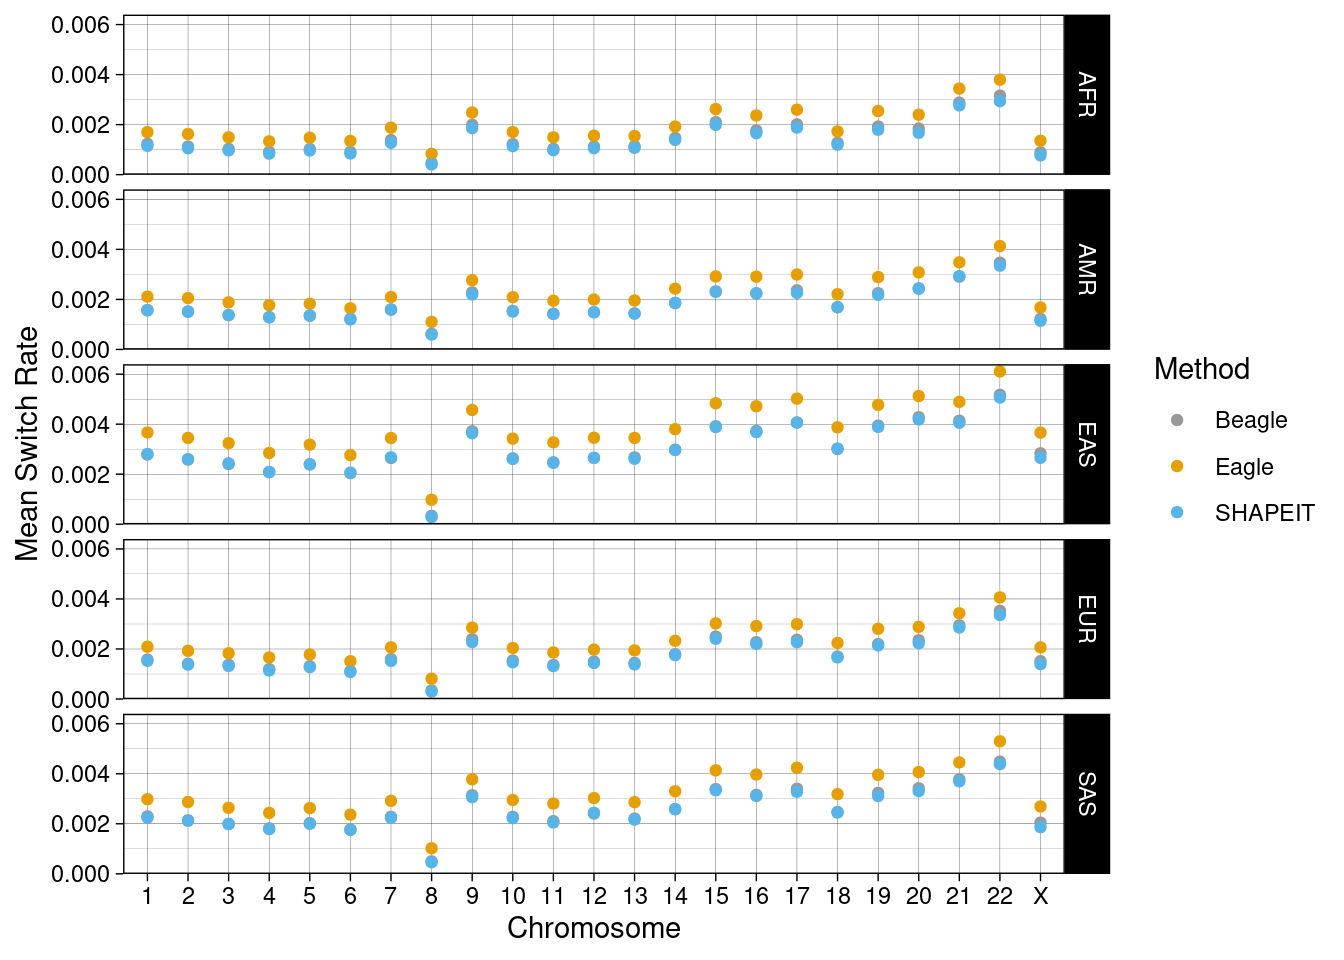
\includegraphics[scale=0.80]{chapters/figures/switch_error_rates_all.png}
    \caption{Average switch error rates by population across all autosomes and chromosome X. While rates vary by chromosome, the ranking of methods is consistent, with Eagle having higer switch error rates than Beagle and SHAPEIT.}
    \label{fig:switch_err}
\end{figure}

In addition to ranking methods by flip and switch error rates, we also evaluate the overlap of errors across methods. Additionally, we assess the distributions of error rates across the chromosomes and correlated these rates by genomic features such as recombination rates, minor allele frequencies, and GC content.